\documentclass[aspectratio=169]{beamer}
\setbeamersize{text margin right=0mm, text margin left=2mm}
\usepackage{graphics}
\usetheme{Pittsburgh}

\usecolortheme{owl}
%Information to be included in the title page:
\title{Titre}
\begin{document}
\begin{frame}
    Vous allez construire une maison jaune avec un toît rouge.
    \vfill
  \begin{center}
      
\includegraphics[width=\linewidth]{figure.png}
  \end{center}
\end{frame}

\begin{frame}
    Étape 1/9
    \vfill
  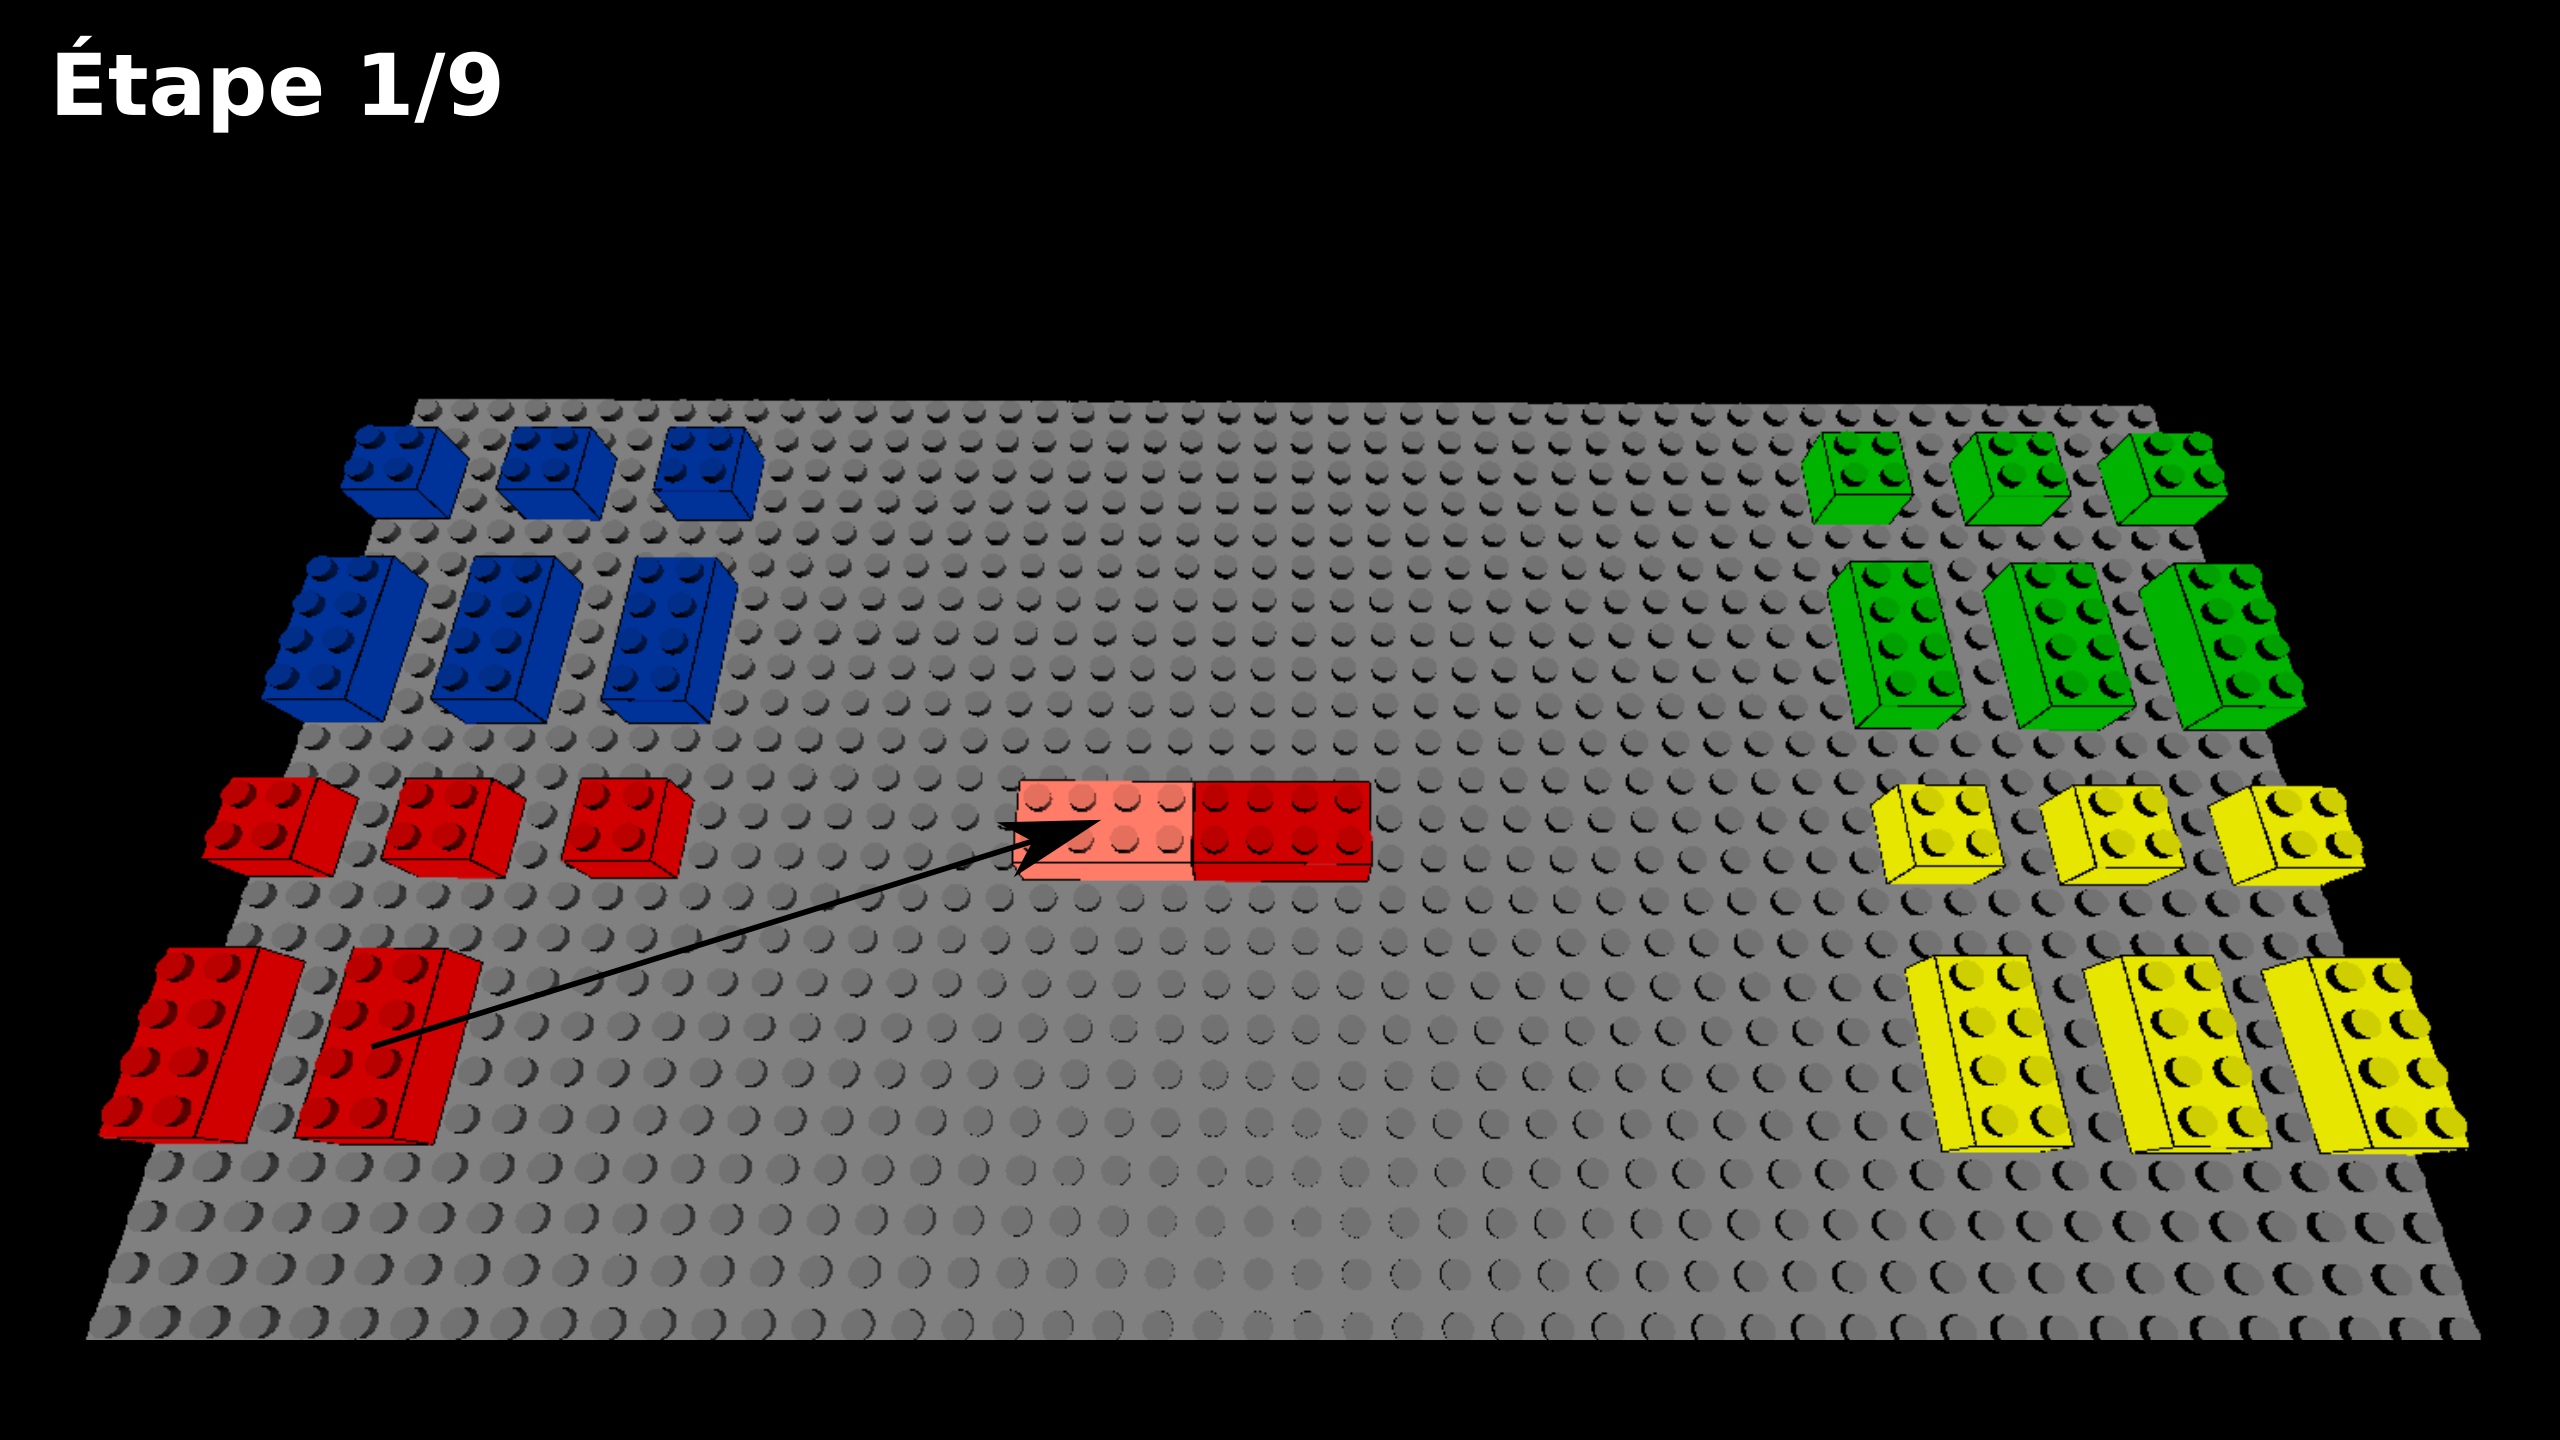
\includegraphics[width=\linewidth]{step1.png}
\end{frame}

\begin{frame}
    Étape 2/9
    \vfill
  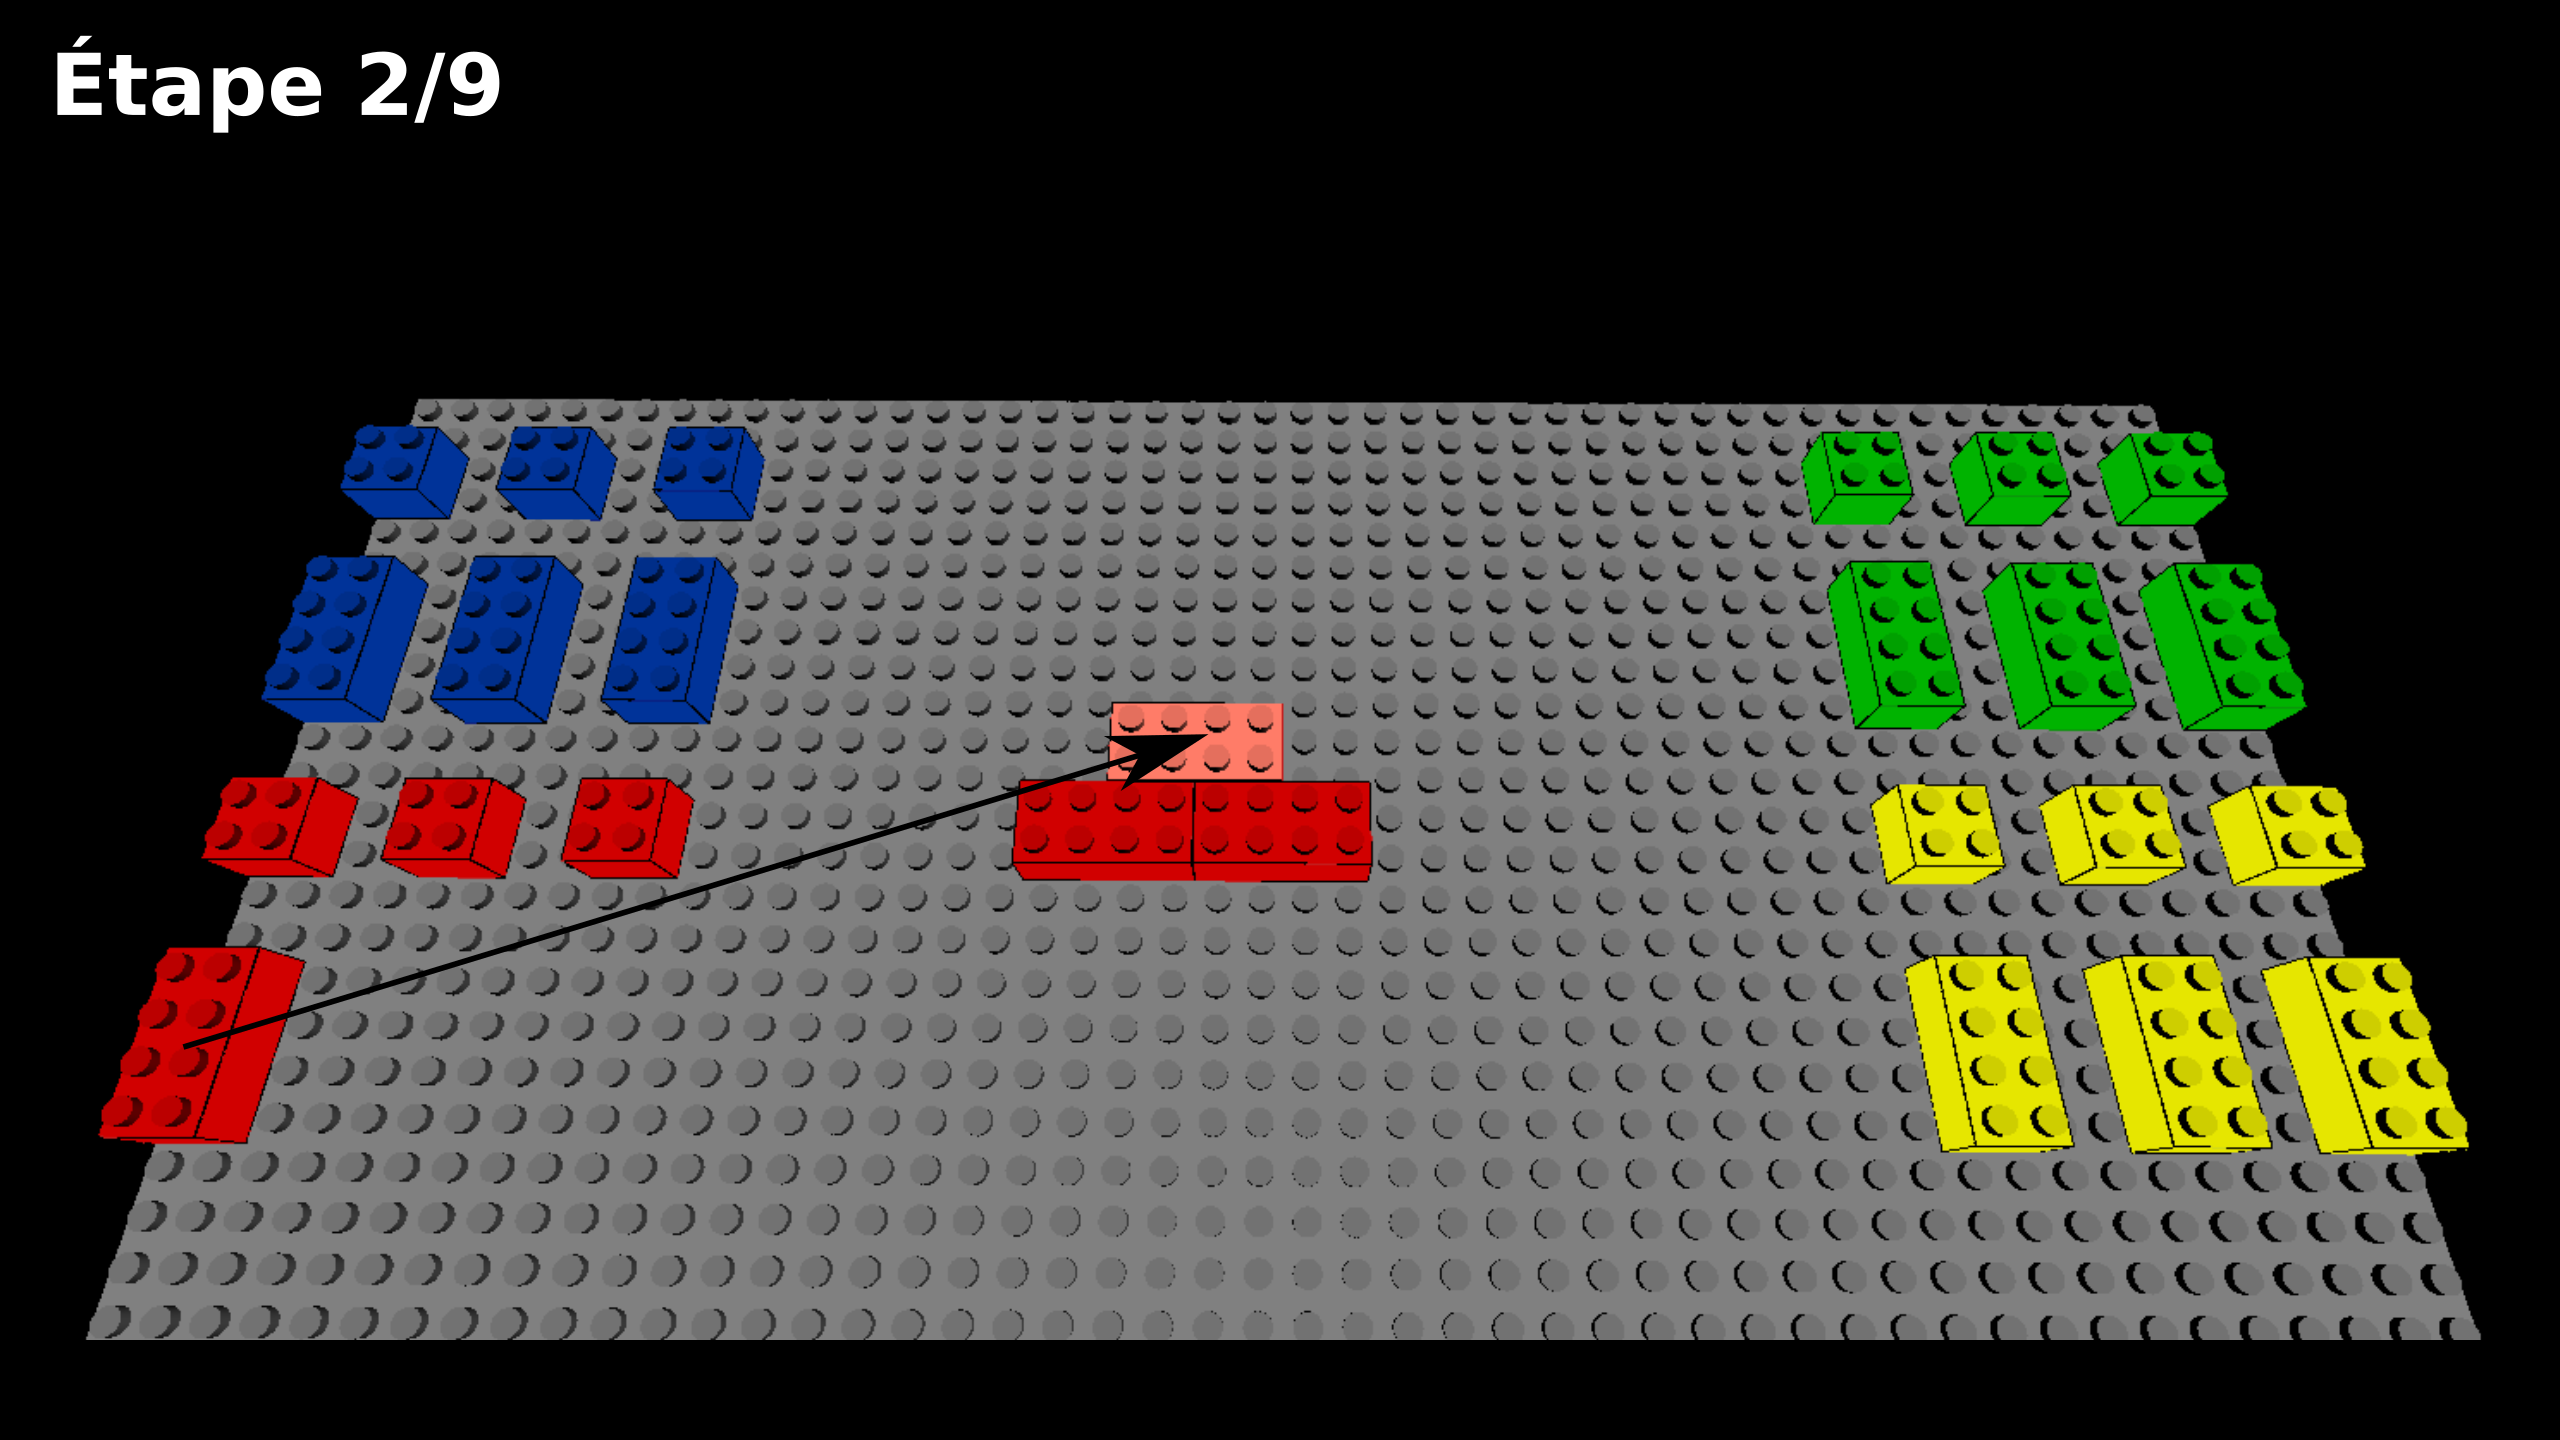
\includegraphics[width=\linewidth]{step2.png}
\end{frame}

\begin{frame}
    Étape 3/9
    \vfill
  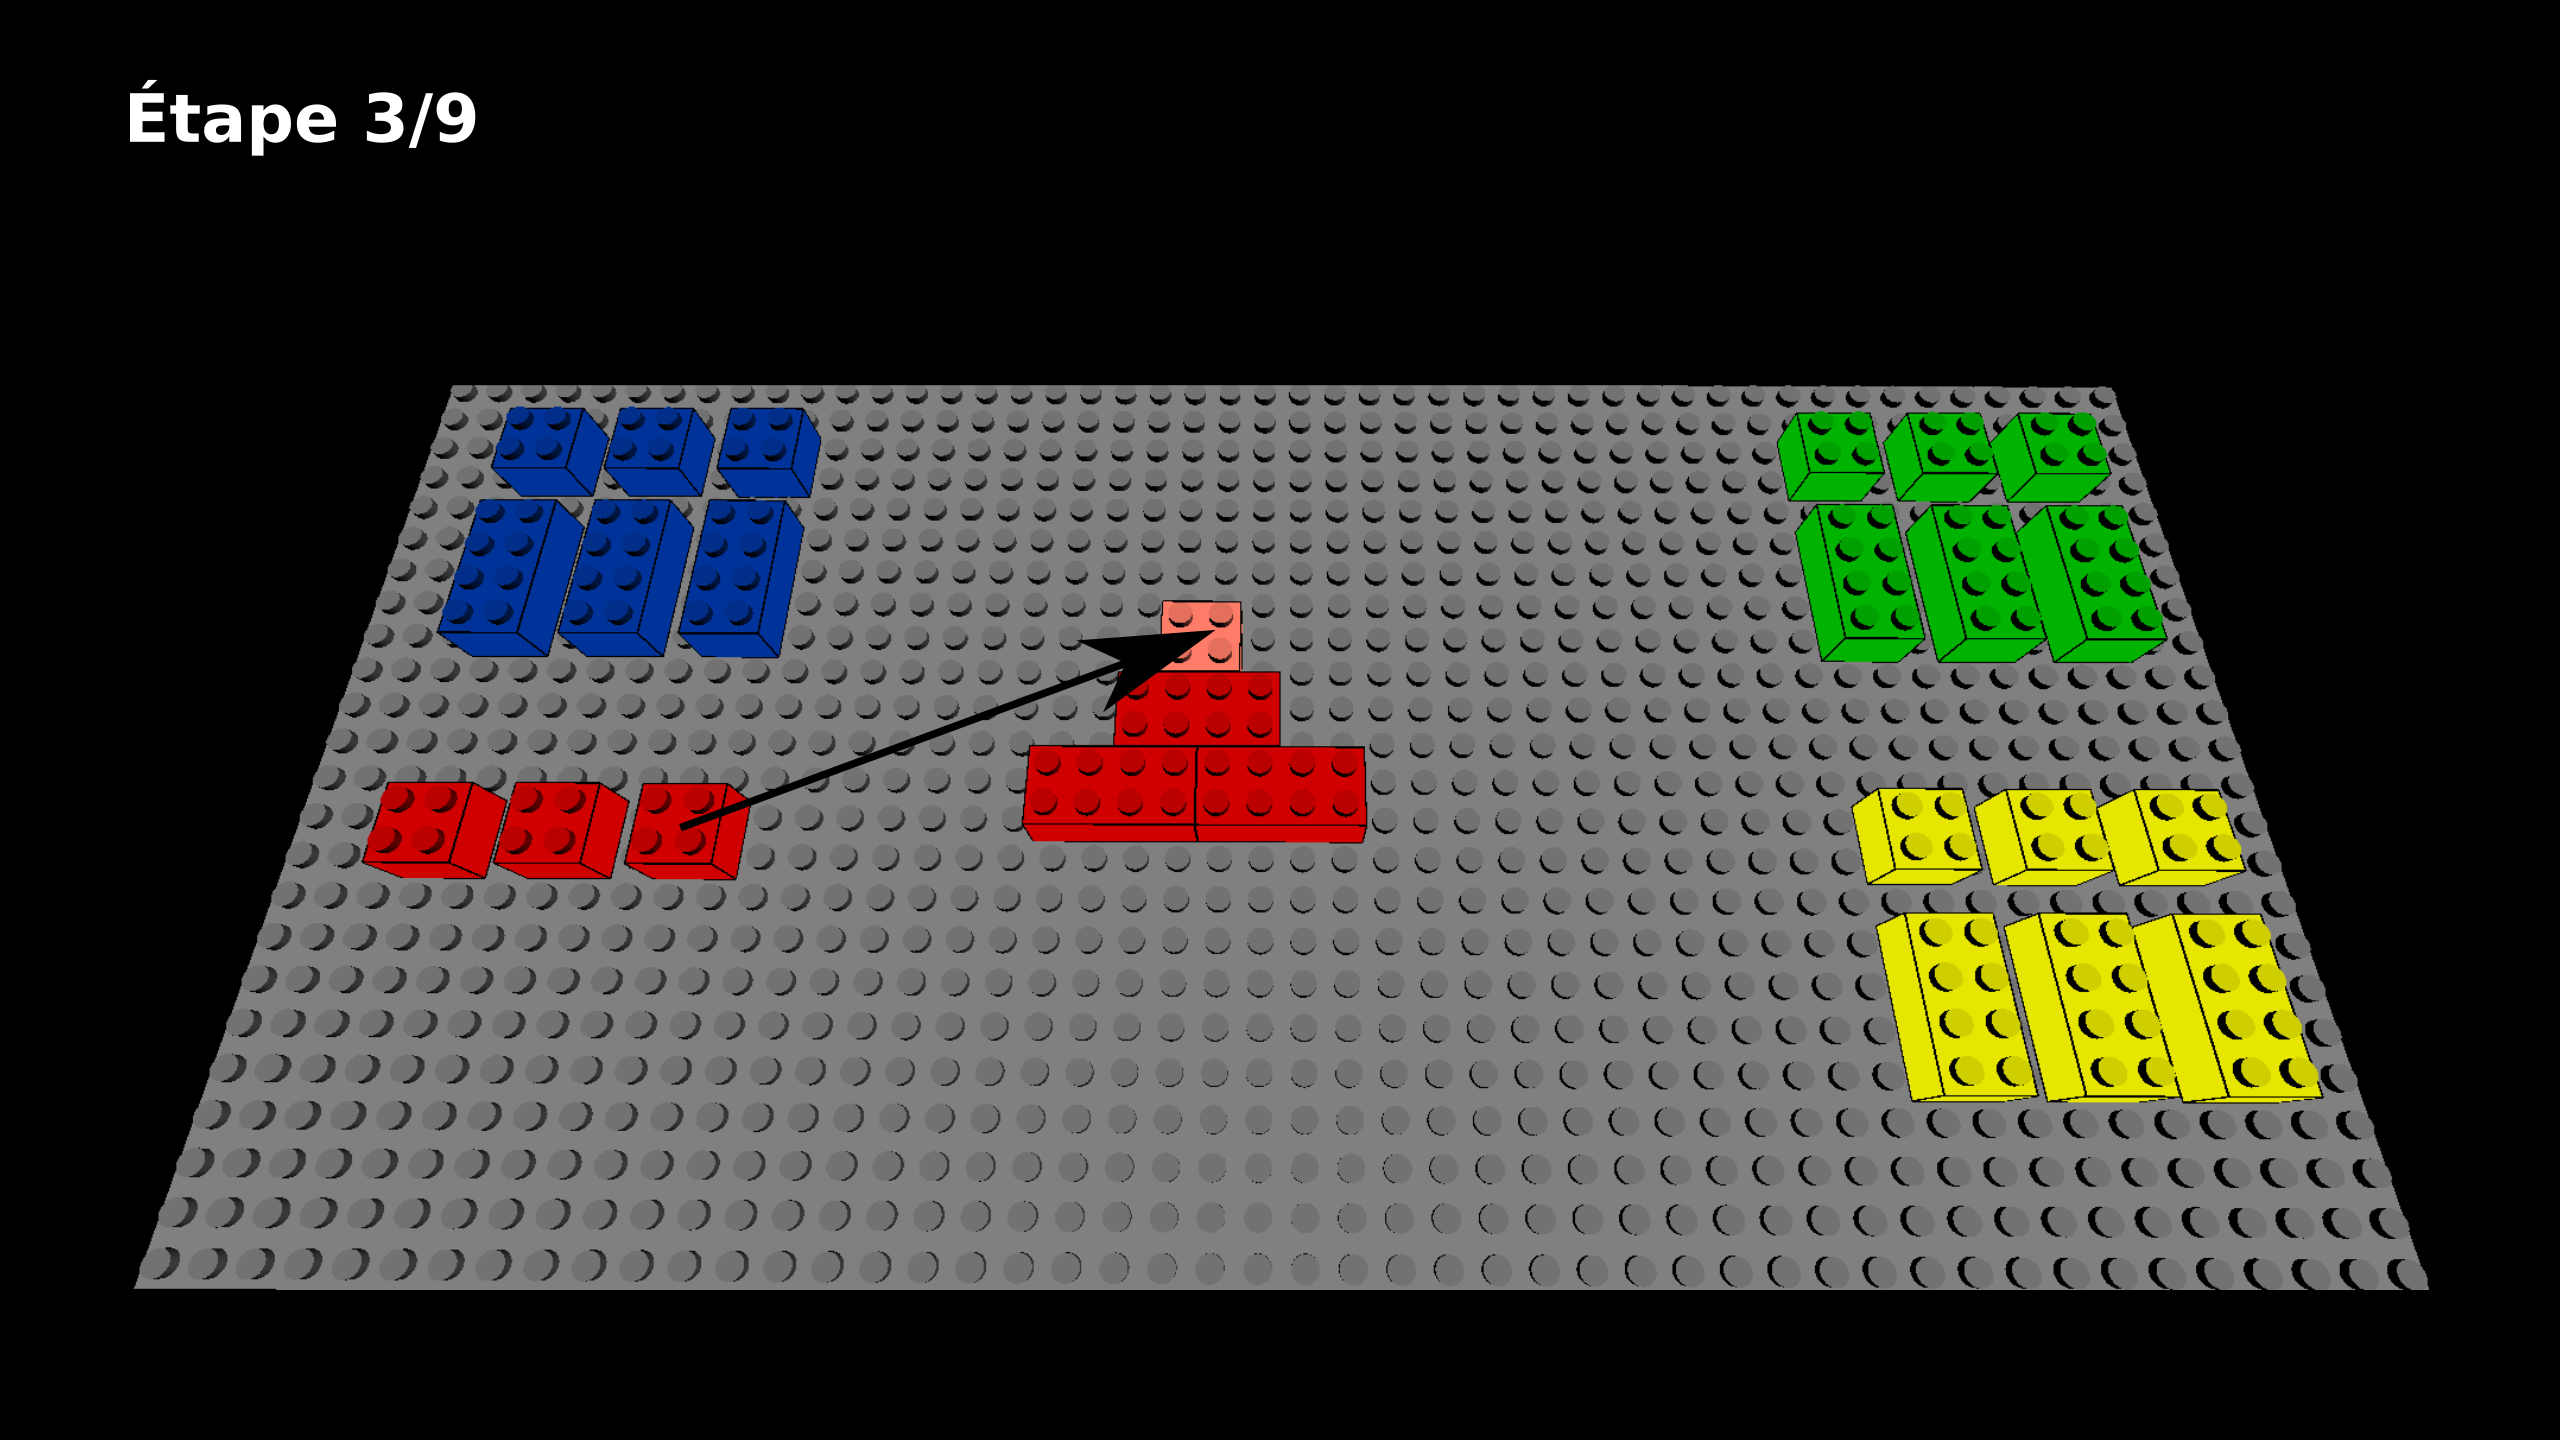
\includegraphics[width=\linewidth]{step3.png}
\end{frame}

\begin{frame}
    Étape 4/9
    \vfill
  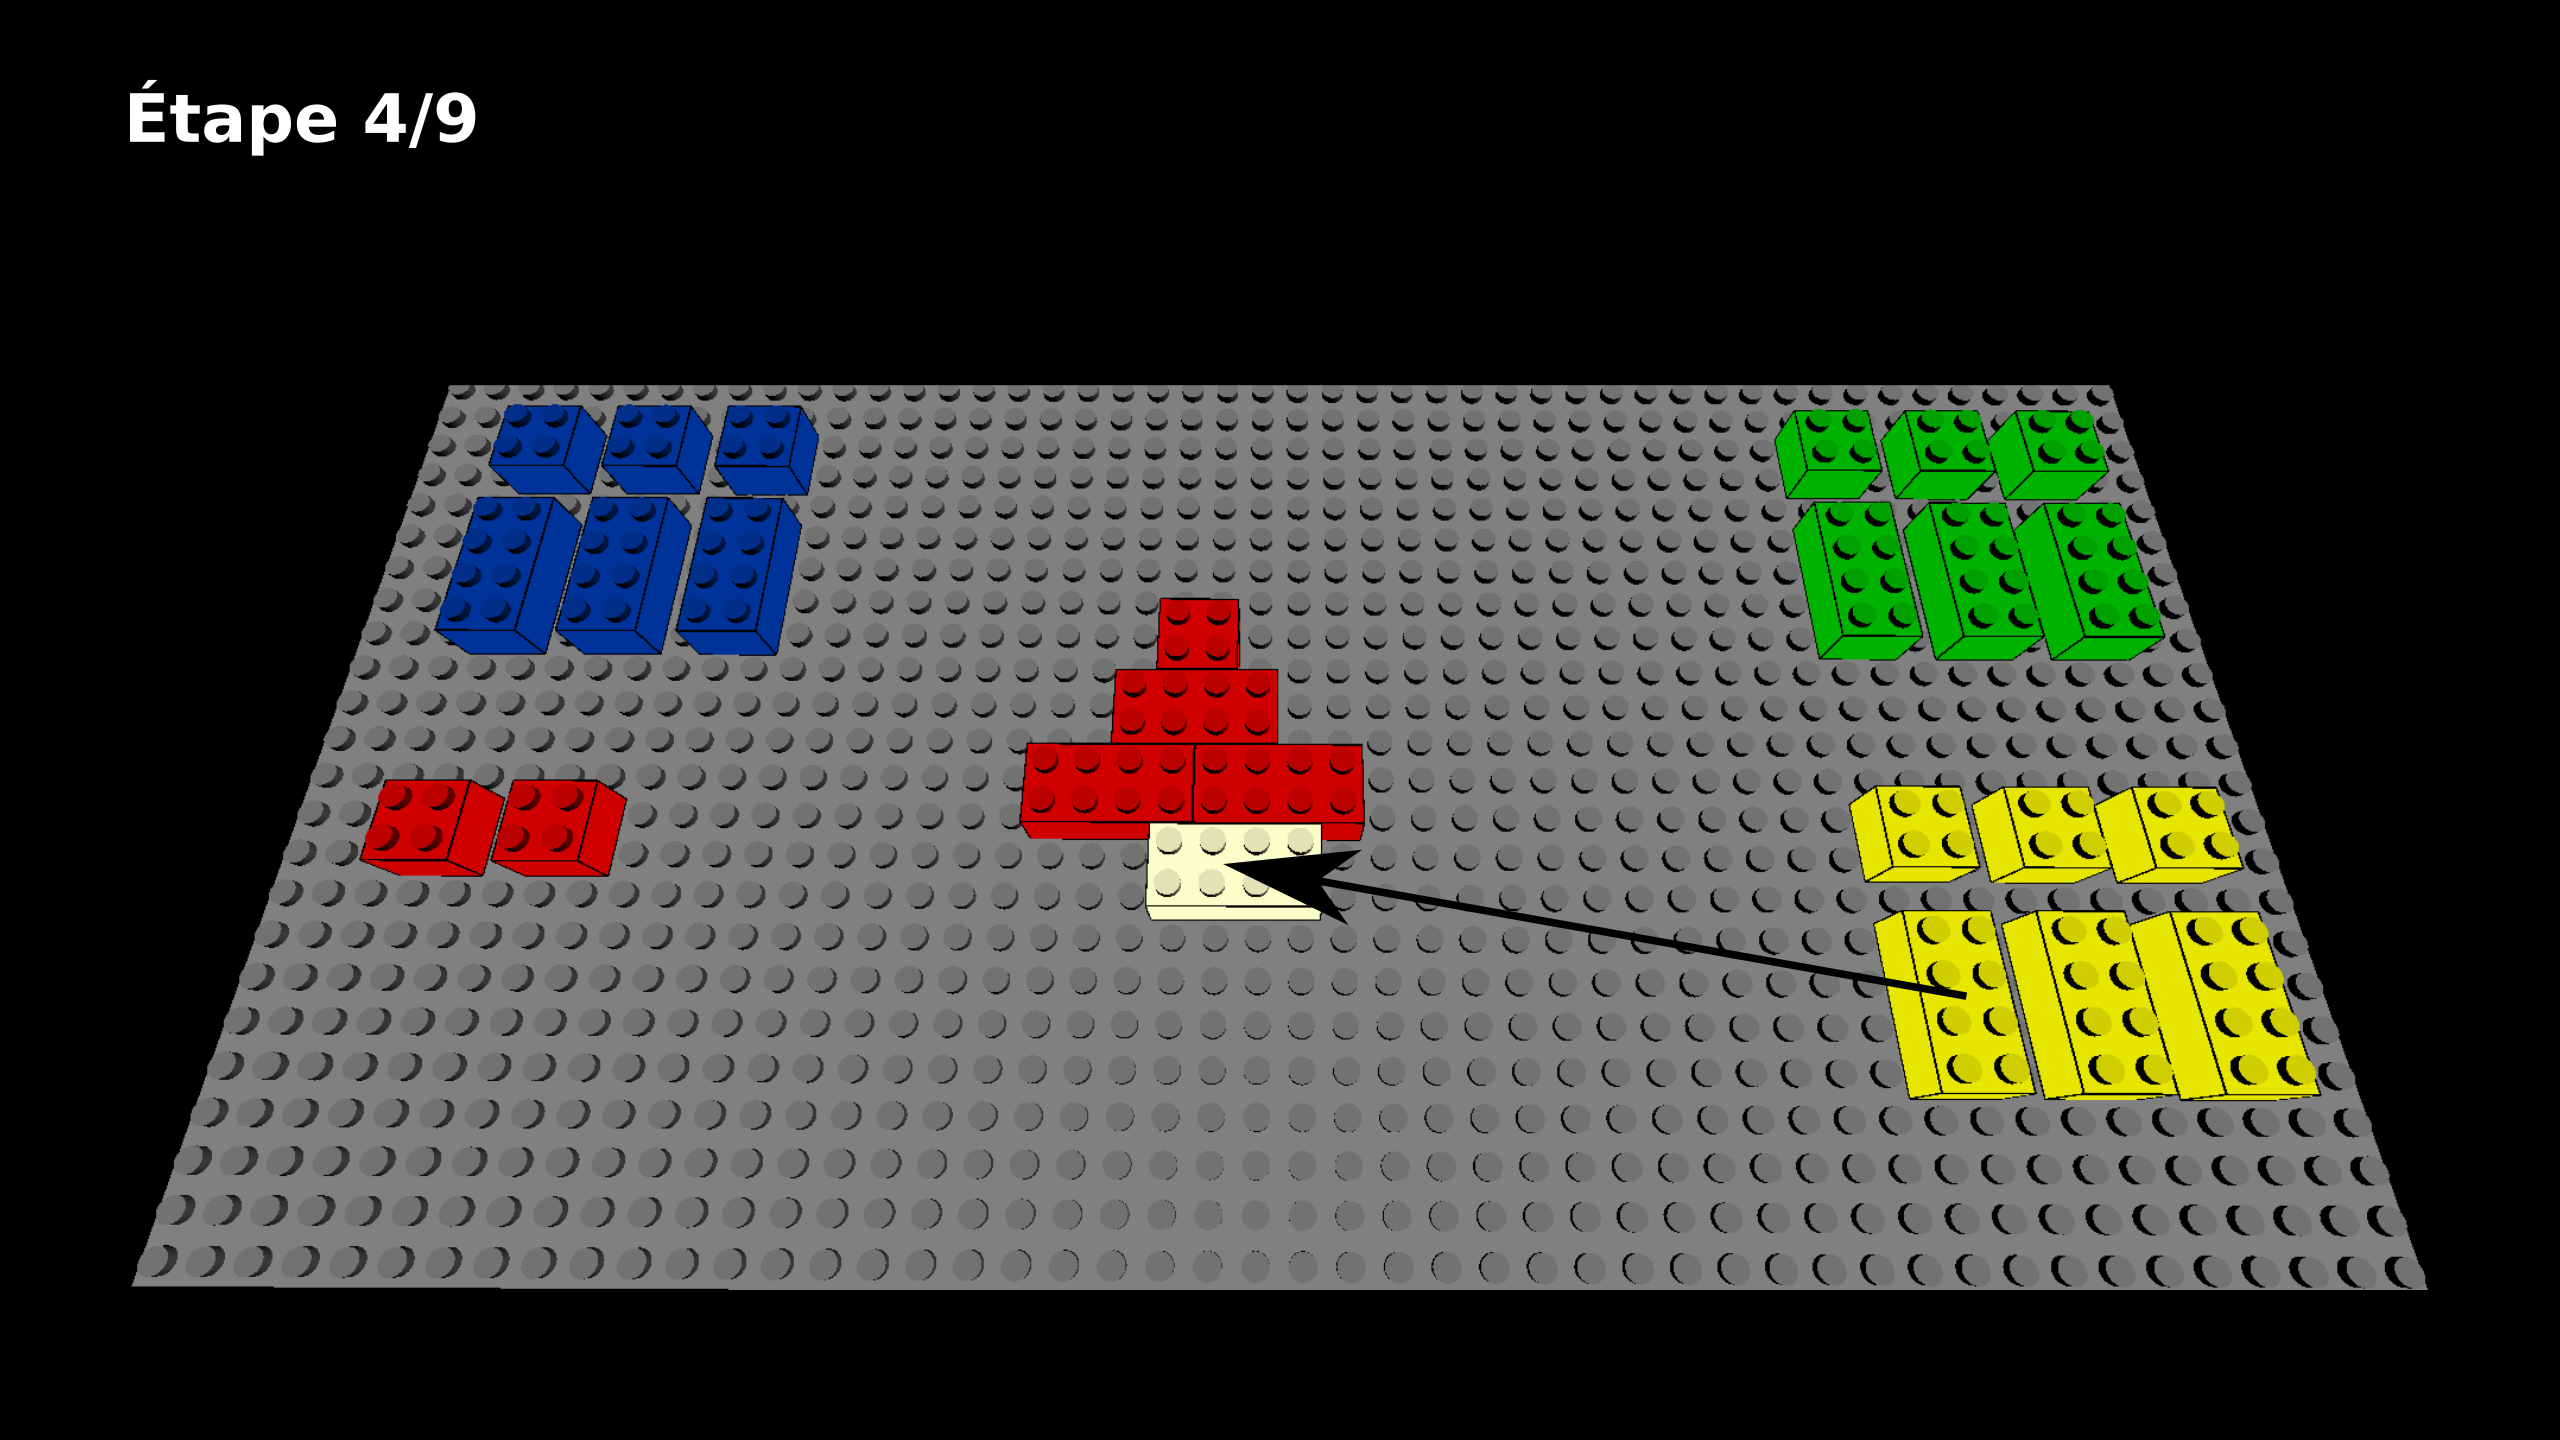
\includegraphics[width=\linewidth]{step4.png}
\end{frame}

\begin{frame}
    Étape 5/9
    \vfill
  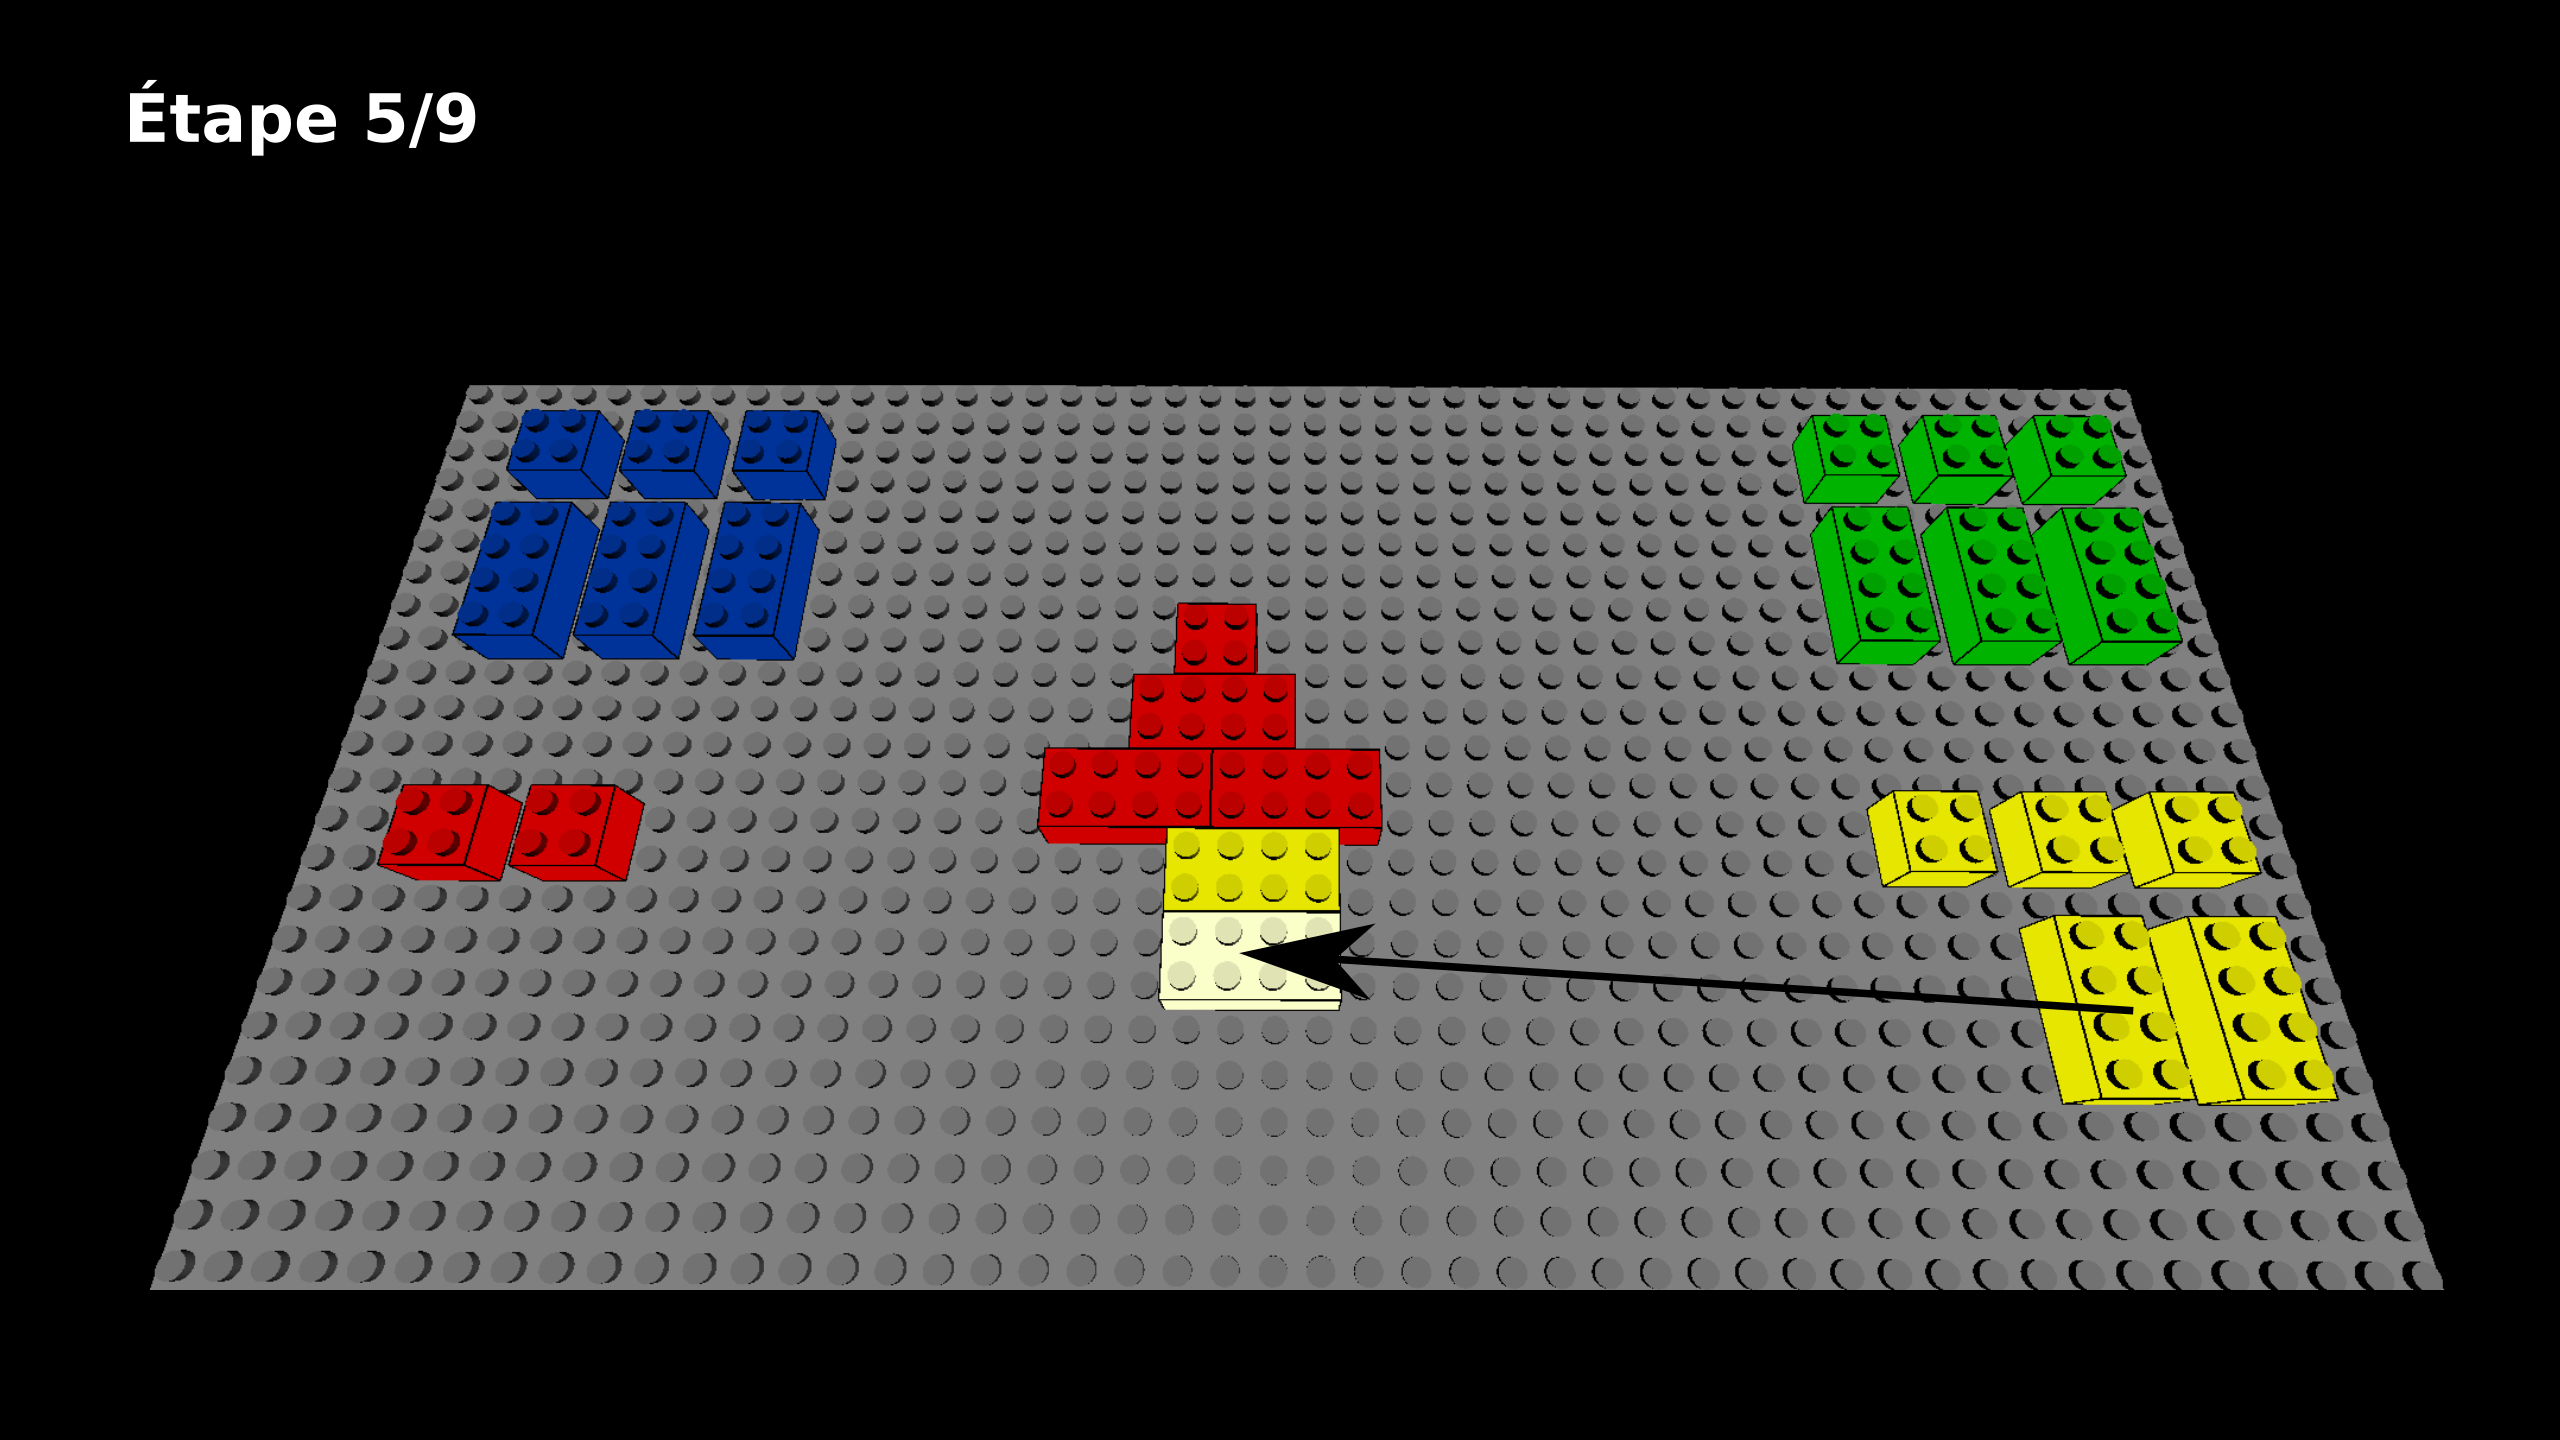
\includegraphics[width=\linewidth]{step5.png}
\end{frame}

\begin{frame}
    Étape 6/9
    \vfill
  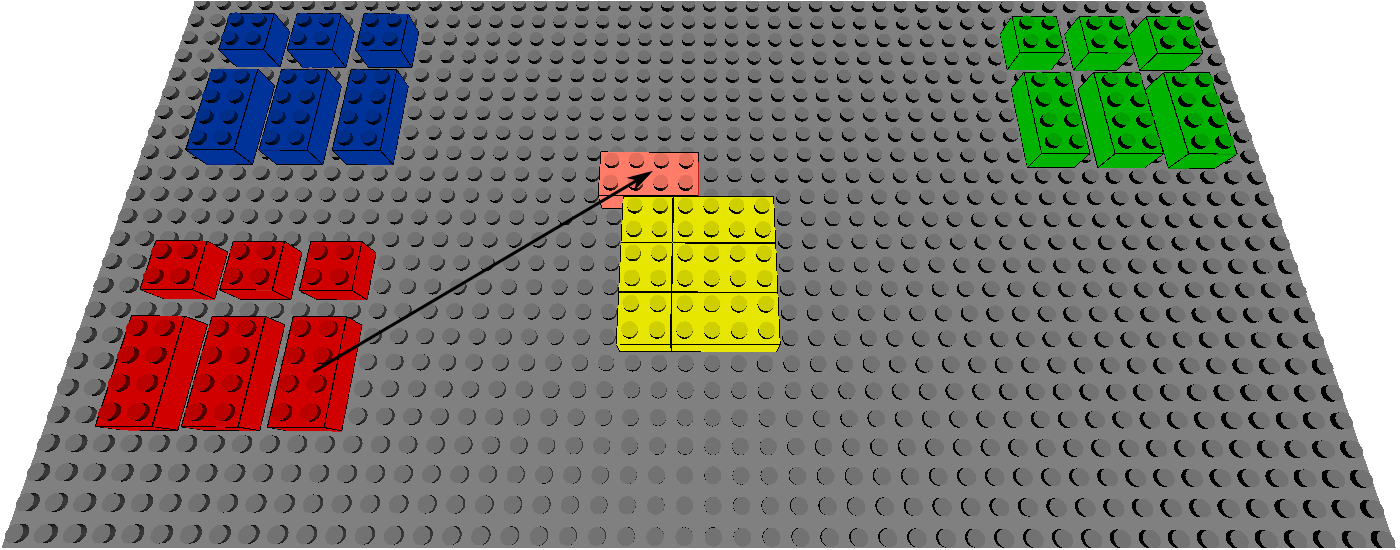
\includegraphics[width=\linewidth]{step6.png}
\end{frame}

\begin{frame}
    Étape 7/9
    \vfill
  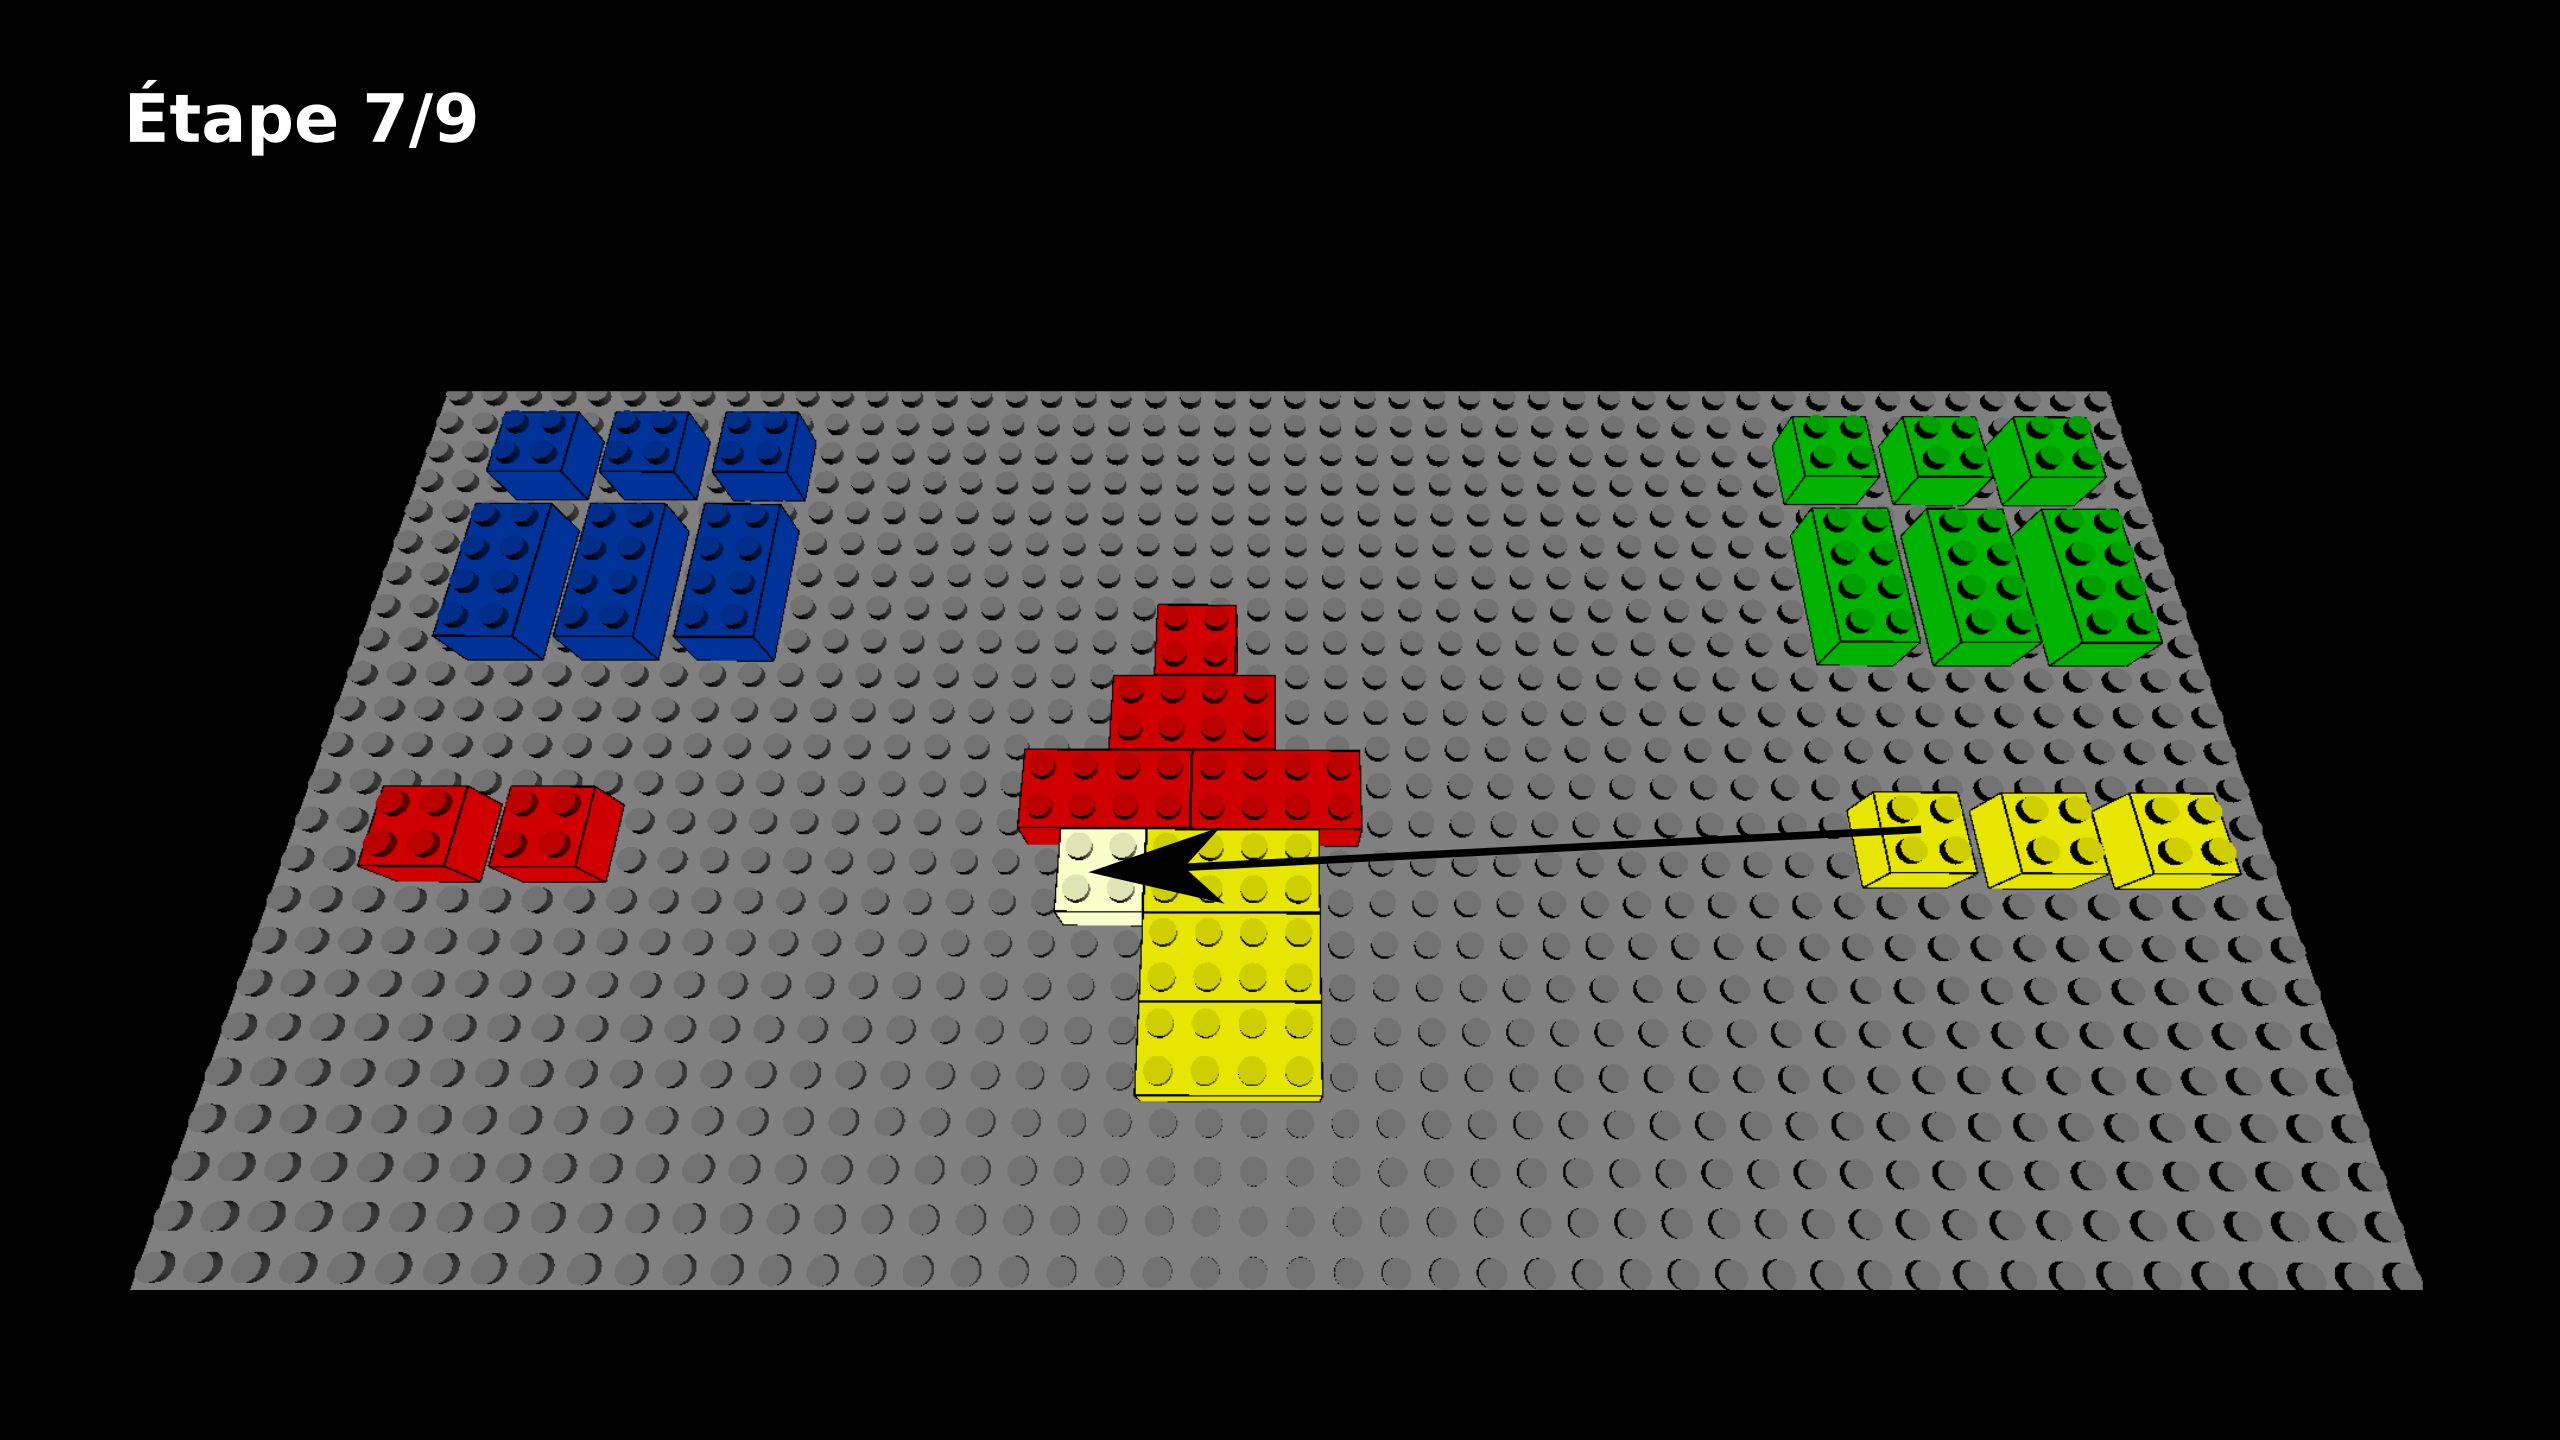
\includegraphics[width=\linewidth]{step7.png}
\end{frame}

\begin{frame}
    Étape 8/9
    \vfill
  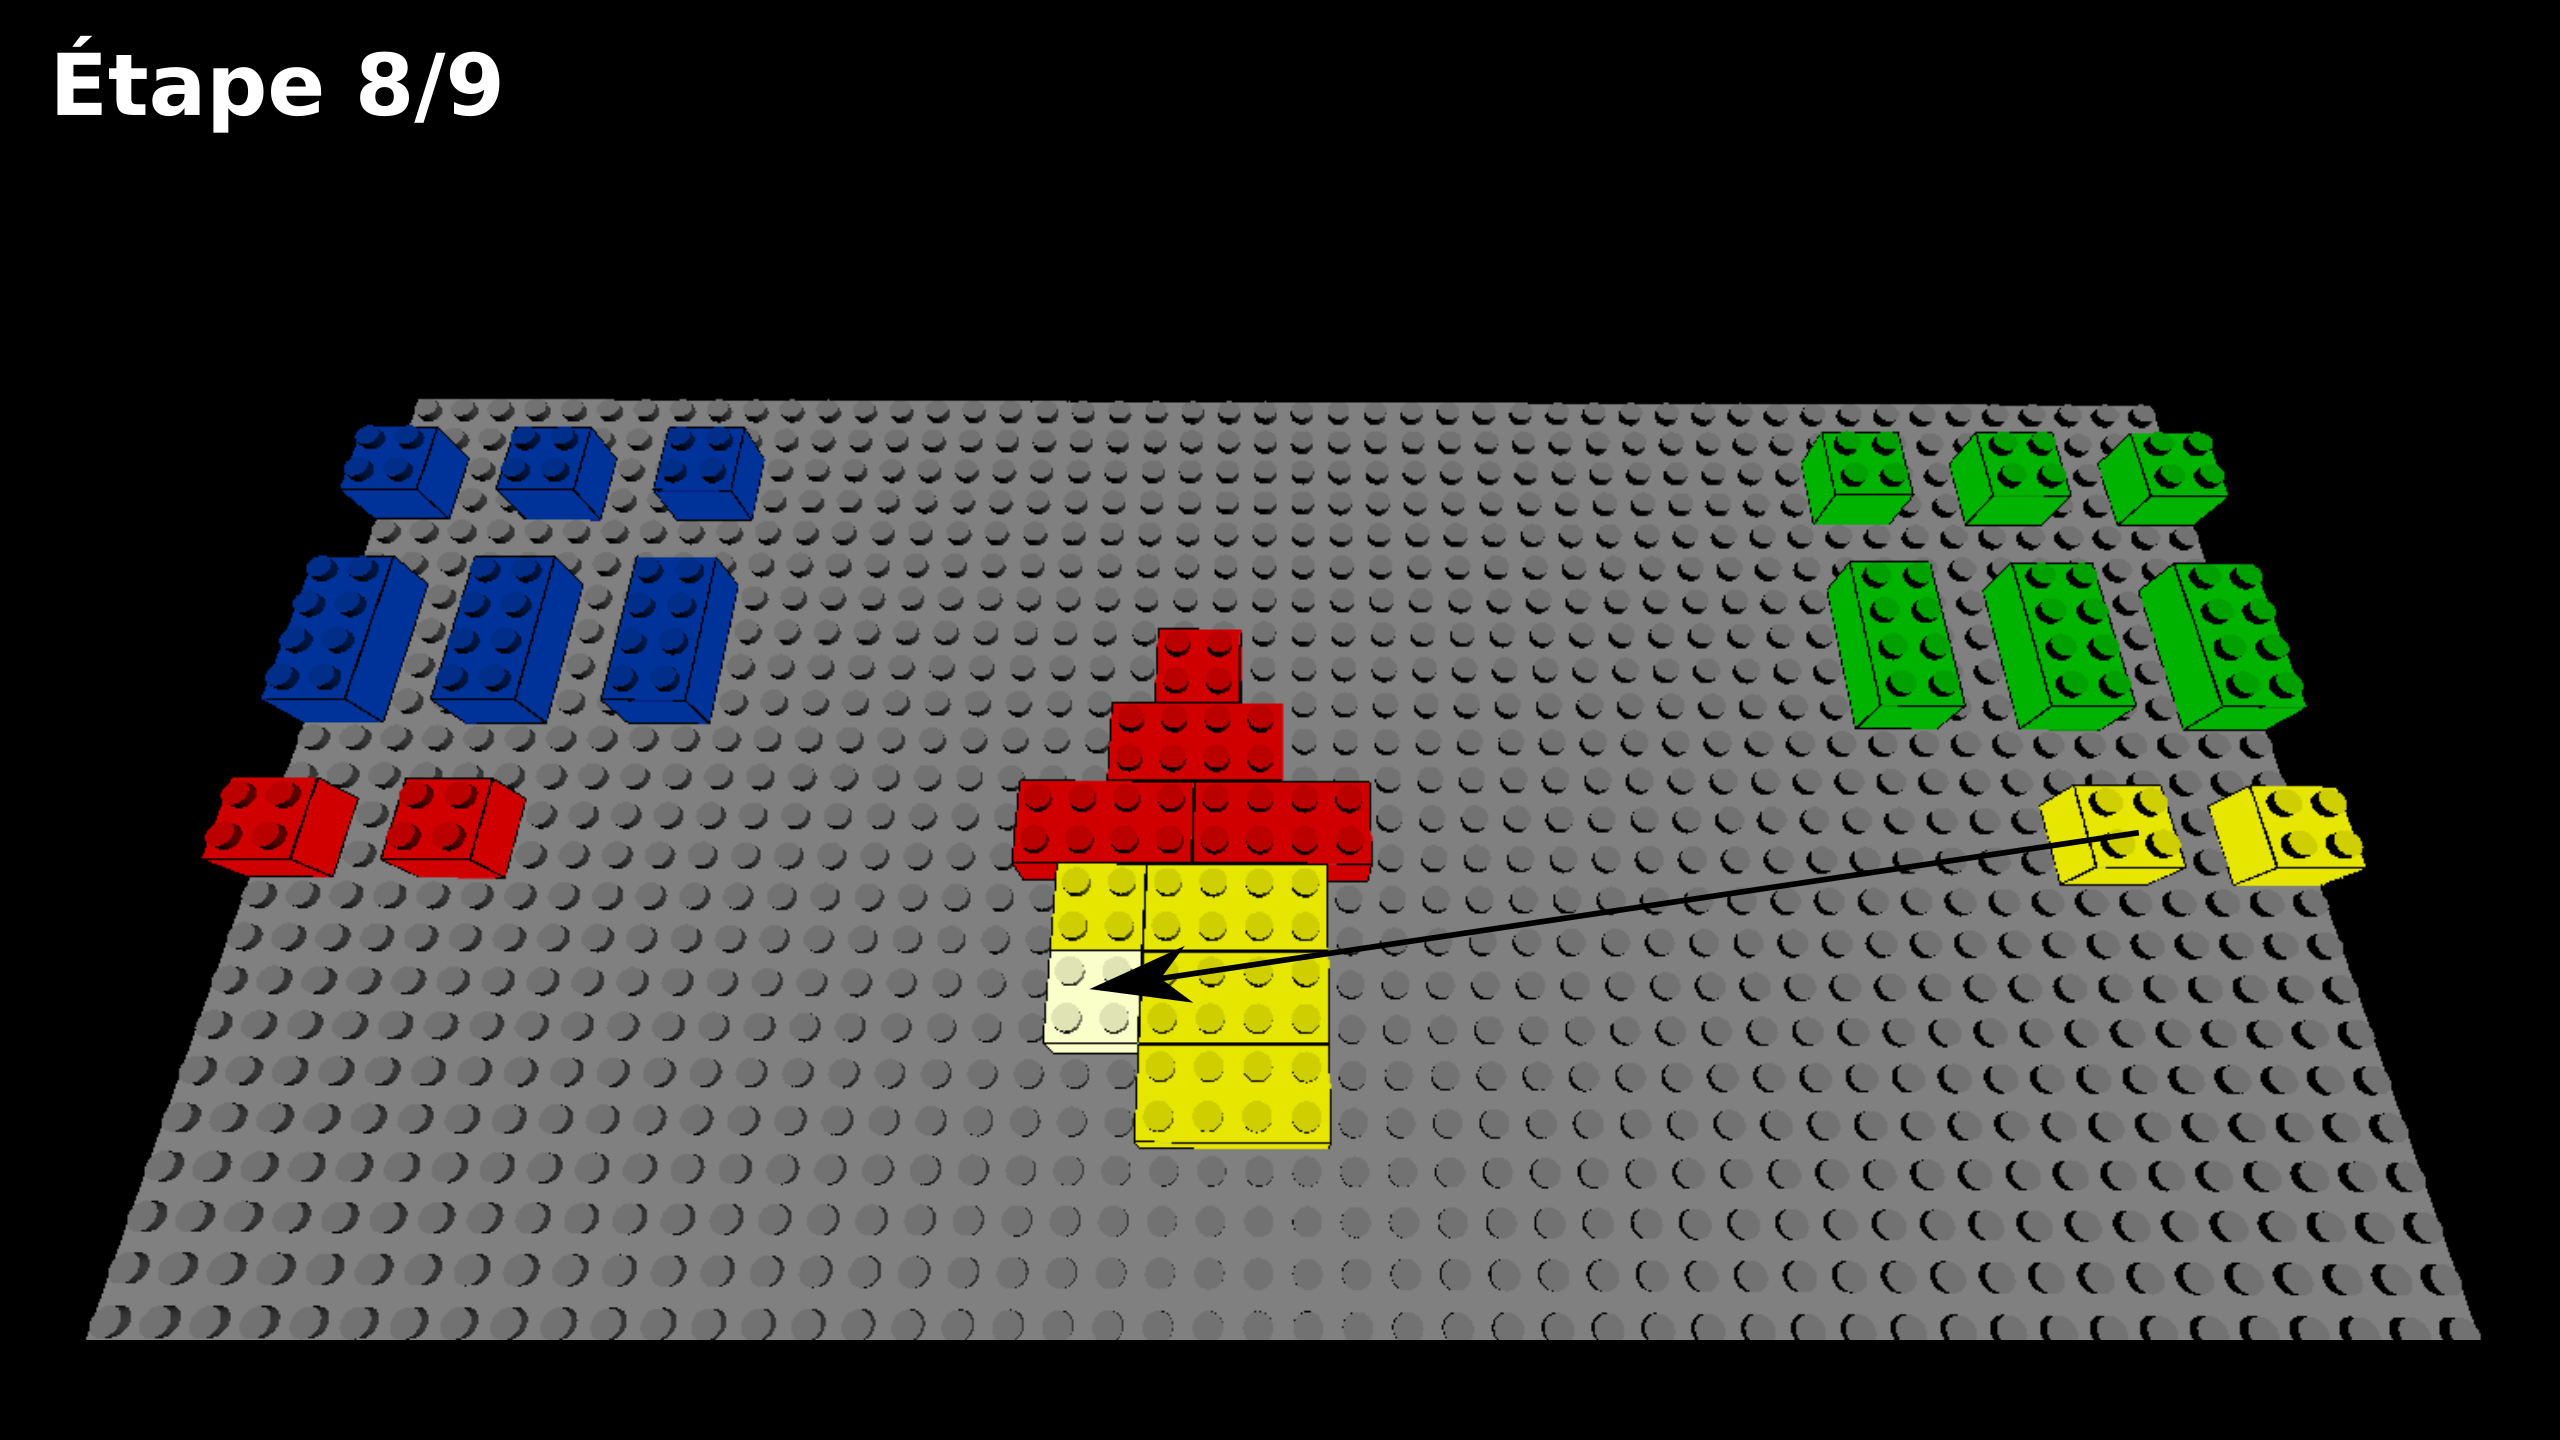
\includegraphics[width=\linewidth]{step8.png}
\end{frame}

\begin{frame}
    Étape 9/9
    \vfill
  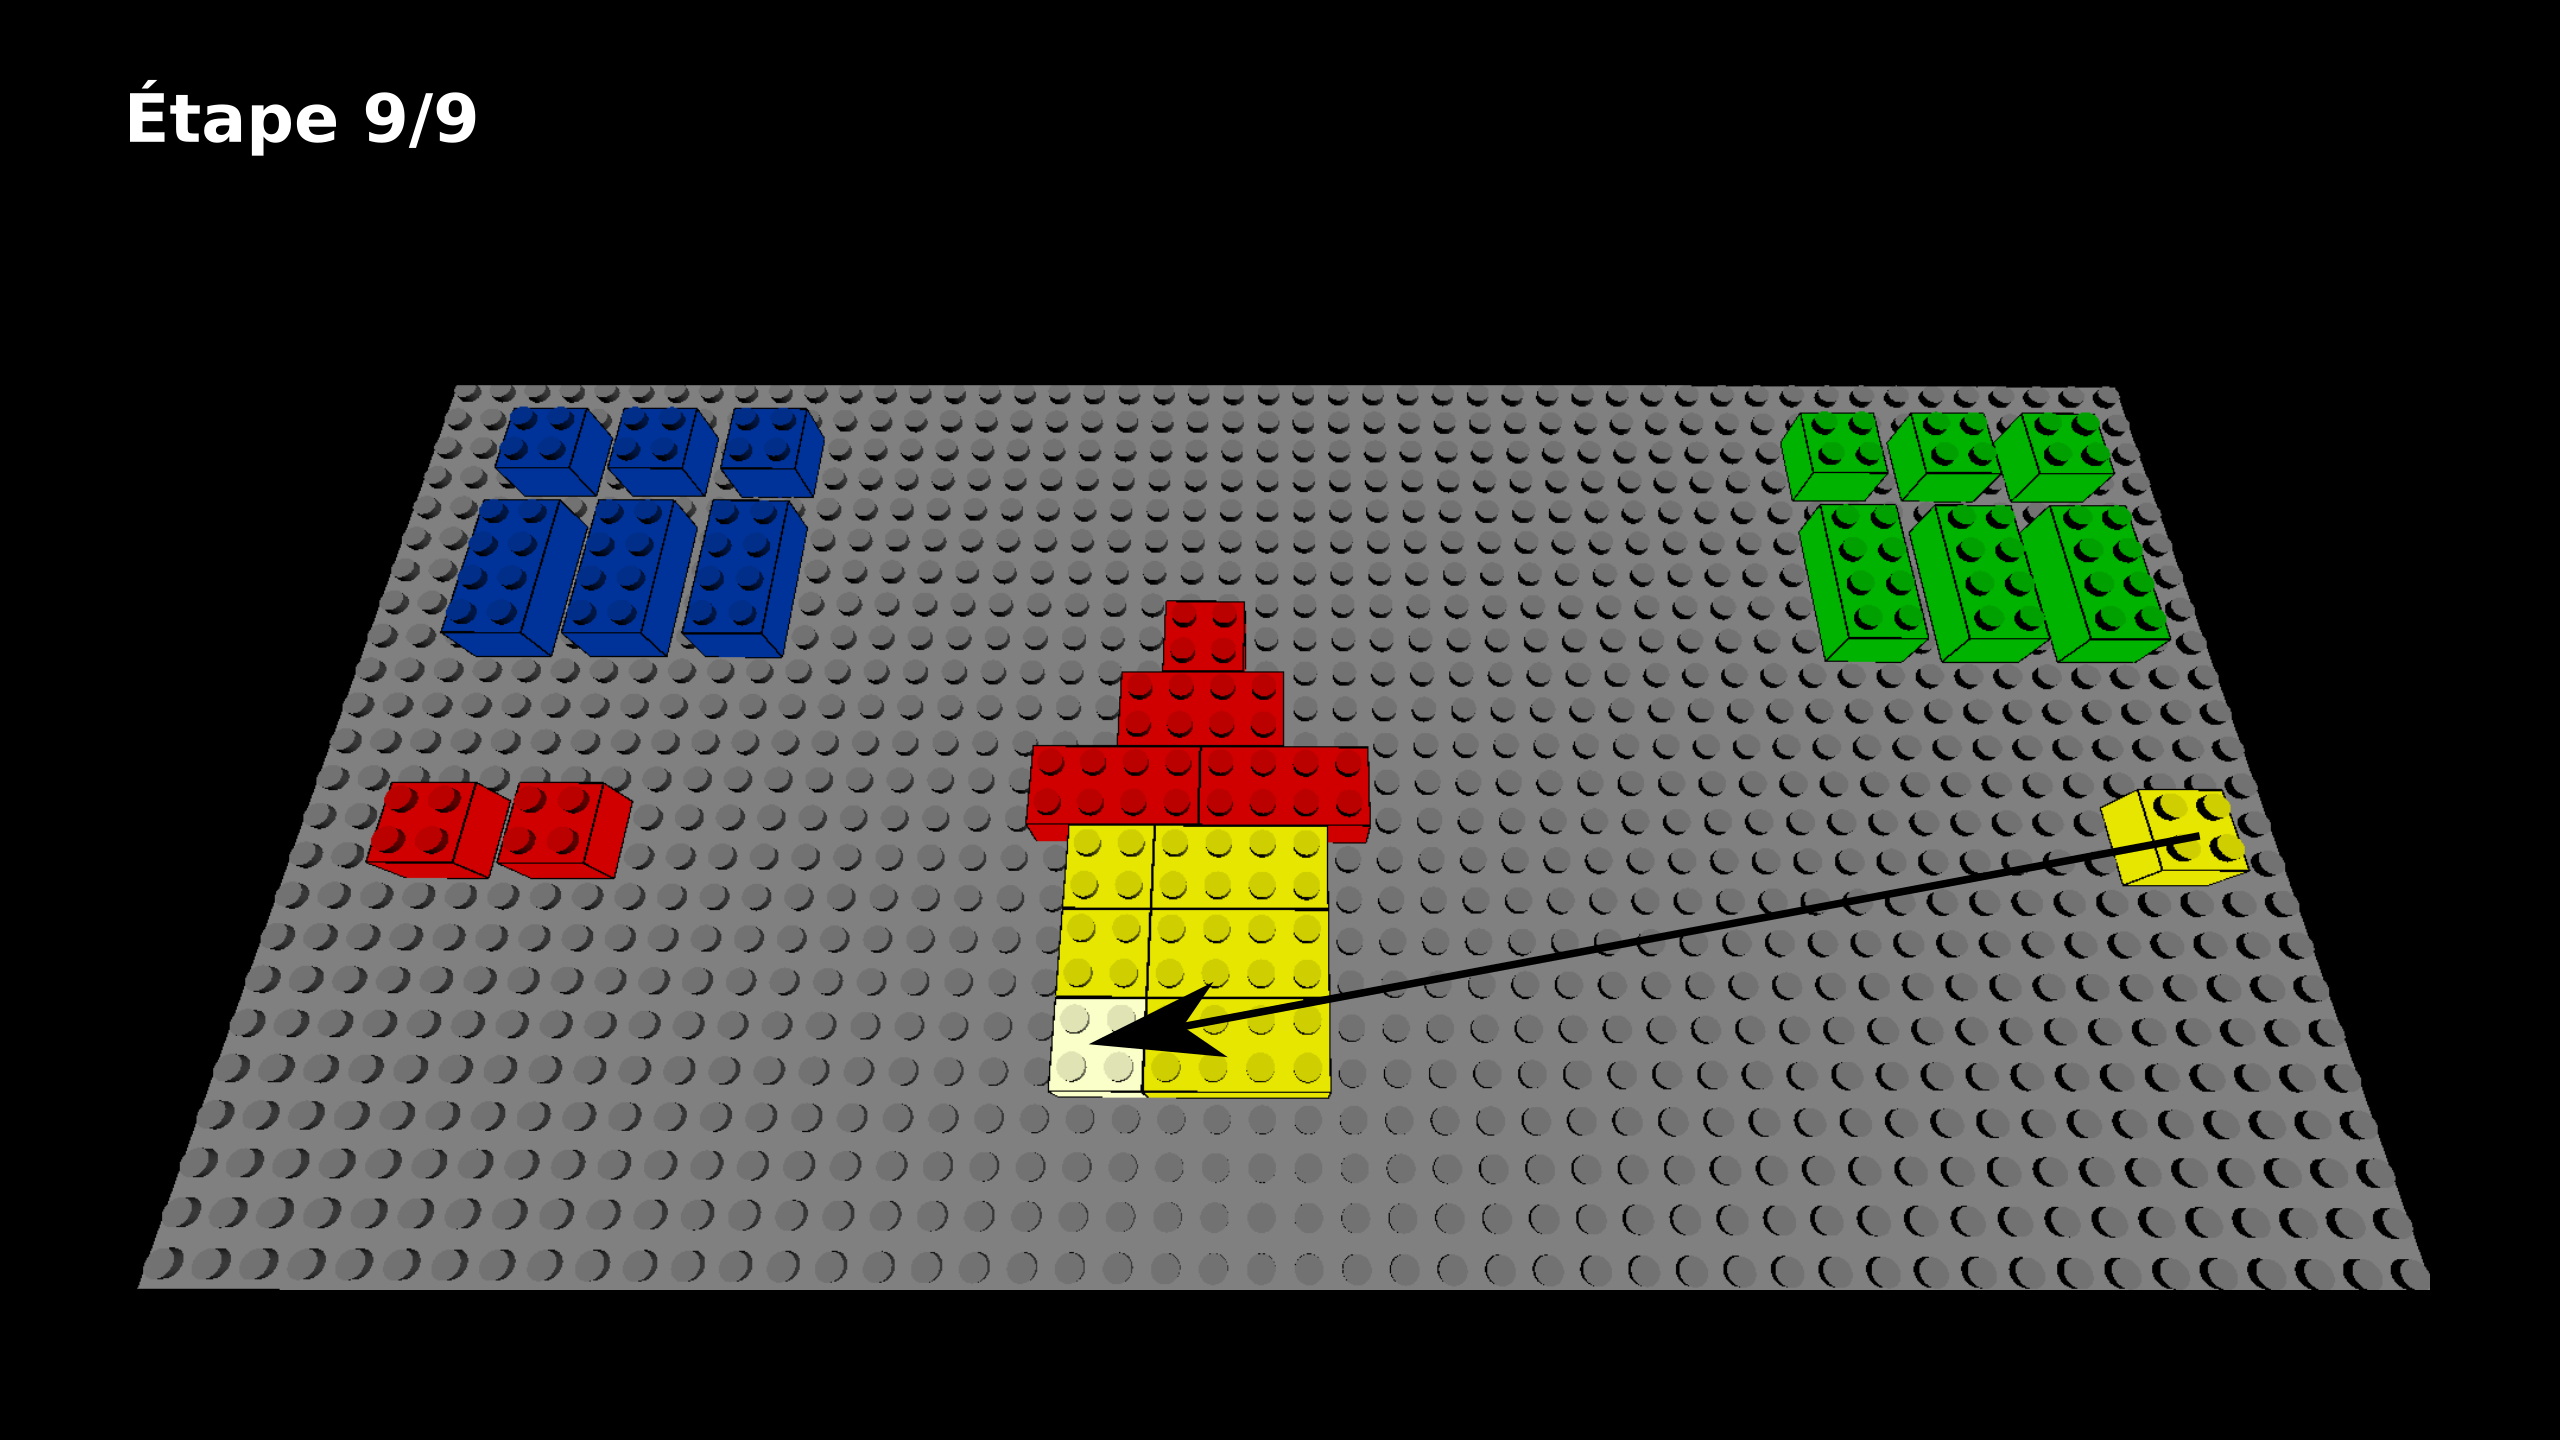
\includegraphics[width=\linewidth]{step9.png}
\end{frame}

\begin{frame}
    Fin.
    \vfill
  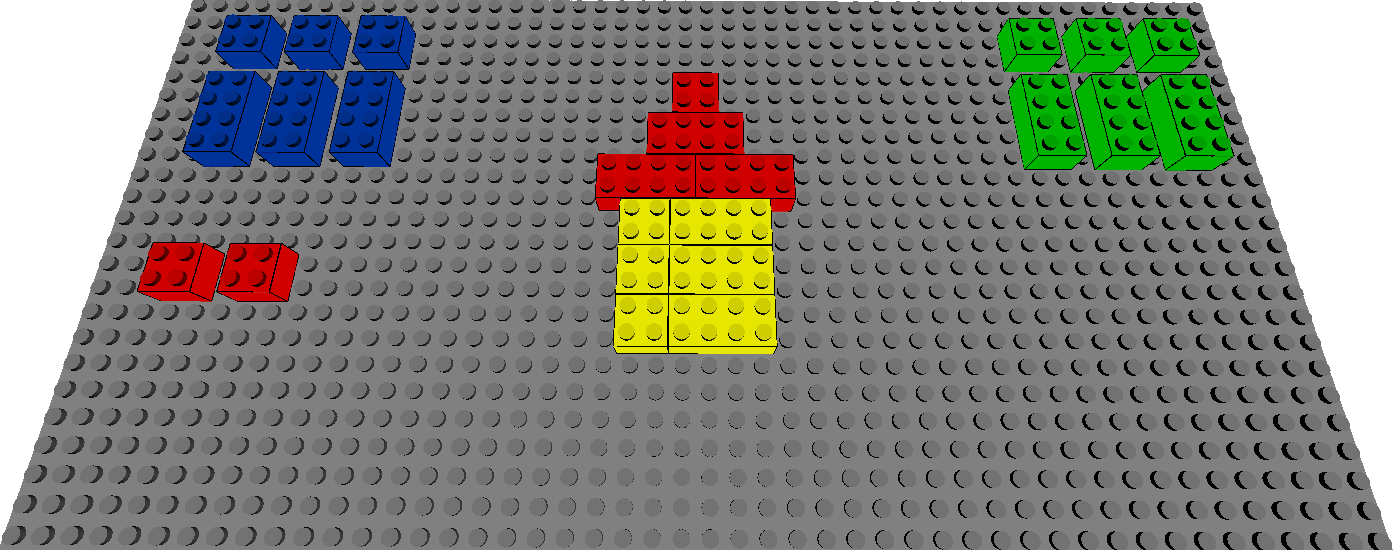
\includegraphics[width=\linewidth]{end.png}
\end{frame}

\end{document}
